\section{Model Description}

\subsection{Introduction}

This module is modeling a VSCMG connected to a rigid body hub. The VSCMG model has three modes that can be ran: balanced wheels, simple jitter, and fully-coupled imbalanced wheels.

The balanced wheels option is modeling the VSCMG as having their principle inertia axes aligned with spin axis, $\hat{\bm g}_s$, and the center of mass of the wheel is coincident with $\hat{\bm g}_s$. This results in the reaction wheel not changing the mass properties of the spacecraft and results in simpler equations. The simple jitter option is approximating the jitter due to mass imbalances by applying an external force and torque to the spacecraft that is proportional to the wheel speeds squared. This is an approximation because in reality this is an internal force and torque. Finally, the fully-coupled mode is modeling VSCMG imbalance dynamics by modeling the static and dynamic imbalances as internal forces and torques which is physically realistic and allows for energy and momentum conservation.

Figure \ref{fig:scplusVSCMG} shows the frame and variable definitions used for this problem. The formulation involves a rigid hub with its center of mass location labeled as point $B_c$, and $N_\text{rw}$ RWs with their center of mass locations labeled as $W_{c_i}$. The frames being used for this formulation are the body-fixed frame, \frameDefinition{B}, the motor frame of the $i^\text{th}$ RW, $\mathcal{M}_i:\{\hat{\bm m}_{s_i},\hat{\bm m}_{2_i},\hat{\bm m}_{3_i}\}$ which is also body-fixed, and the wheel-fixed frame of the $i^\text{th}$ RW, $\mathcal{W}_i:\{\hat{\bm g}_{s_i},\hat{\bm w}_{2_i},\hat{\bm w}_{3_i}\}$. The dynamics are modeled with respect to the $\mathcal{B}$ frame which can be generally oriented. The $\mathcal{W}_i$ frame is oriented such that the $\hat{\bm g}_{s_i}$ axis is aligned with the RW spin axis  which is the same as the motor torque axis $\hat{\bm m}_{s_{i}}$, the $\hat{\bm w}_{2_i}$ axis is perpendicular to $\hat{\bm g}_{s_i}$ and points in the direction towards the RW center of mass $W_{c_i}$. The $\hat{\bm w}_{3_i}$ completes the right hand rule. The $\mathcal{M}_i$ frame is defined as being equal to the $\mathcal{W}_i$ frame at the beginning of the simulation and therefore the $\mathcal{W}_i$ and $\mathcal{M}_i$ frames are offset by an angle, $\theta_i$, about the $\hat{\bm m}_{s_i} = \hat{\bm g}_{s_i}$ axes.
	
A few more key variables in Figure~\ref{fig:scplusVSCMG} need to be defined. The rigid spacecraft structure without the VSCMGs is called the hub.  Point $B$ is the origin of the $\mathcal{B}$ frame and is a general body-fixed point that does not have to be identical to the total spacecraft center of mass, nor the rigid hub center of mass $B_{c}$. Point $W_i$ is the origin of the $\mathcal{W}_i$ frame and can also have any location relative to point $B$. Point $C$ is the center of mass of the total spacecraft system including the rigid hub and the VSCMGs. Due to the VSCMG imbalance, the vector $\bm c$, which points from point $B$ to point $C$, will vary as seen by a body-fixed observer. The scalar variable $d_i$ is the center of mass offset of the VSCMG, or the distance from the spin axis, $\hat{\bm g}_{\text{s}_i}$ to $W_{c_i}$.  Finally, the inertial frame orientation is defined through $\frameDefinition{N}$, while the origin of the inertial frame is labeled as $N$.

\begin{figure}[htbp]
	\centerline{
		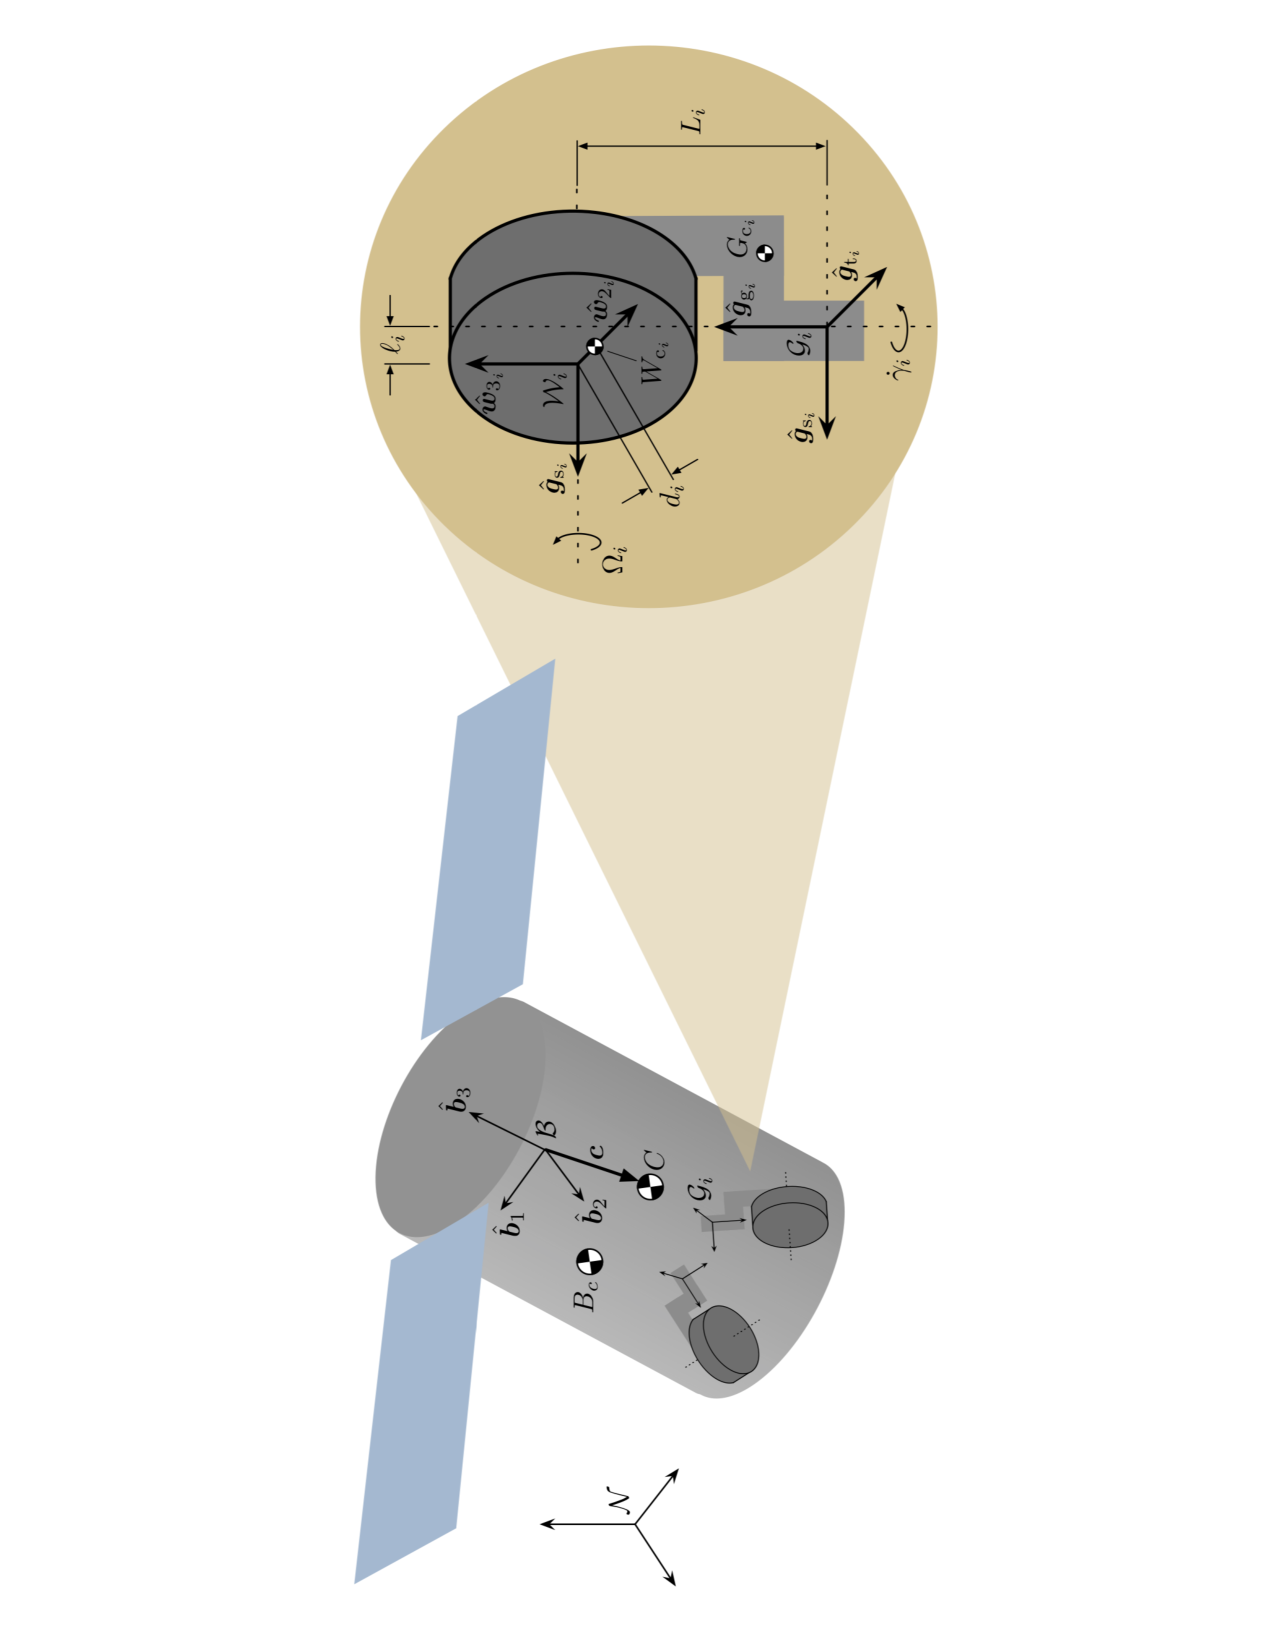
\includegraphics[angle=-90,width=0.8\textwidth]{Figures/scplusVSCMG}}
	\caption{VSCMG and spacecraft frame and variable definitions}
	\label{fig:scplusVSCMG}
\end{figure}

\subsection{Equations of Motion}

The main introduction that is needed for this model is the equations of motion. Depending on the mode, the equations of motion are different. Each mode's equations of motion are discussed in the following sub sections.

\subsubsection{Translational EOMs}
\begin{multline}
	\ddot{\bm r}_{B/N} - [\tilde{\bm{c}}]\dot{\bm \omega} 
	+ \frac{1}{m_{\text{sc}}} \sum\limits_{i=1}^{N} \left[ m_{\text{G}_i}\left[\tilde{\hat{\bm g}}_{\text{g}_i}] \bm{r}_{G_{c_i}/G_i} - m_{\text{W}_i}d_i\c\theta_i\hat{\bm{g}}_{\text{s}_i} + m_{\text{W}_i}\ell_i\hat{\bm{g}}_{\text{t}_i} \right] \ddot{\gamma}_i
	+ \frac{1}{m_{\text{sc}}} \sum\limits_{i=1}^{N} \left[ m_{\text{W}_i}d_i\hat{\bm w}_{3_i} \right]\dot{\Omega}_i
	\\= \ddot{\bm r}_{C/N} - 2[\tilde{\bm{\omega}}]\bm{c}' - [\tilde{\bm{\omega}}][\tilde{\bm{\omega}}]\bm{c} 
	- \frac{1}{m_{\text{sc}}} \sum\limits_{i=1}^{N} \Big[ 
	m_{\text{G}_i}\dot{\gamma}_i[\tilde{\hat{\bm g}}_{\text{g}_i}] \bm{r}_{G_{c_i}/B}'
	\\+ m_{\text{W}_i} \big[ \left(2d_i\dot{\gamma}_i\Omega_i\text{s}\theta_i - \ell_i\dot{\gamma}_i^2\right)\hat{\bm{g}}_{\text{s}_i} - d_i\dot{\gamma}_i^2\c\theta_i\hat{\bm{g}}_{\text{t}_i} - d_i\Omega_i^2 \hat{\bm{w}}_{2_i} \big] \Big]
\end{multline}
This equation represents 3 DOF and contains all second order states ($\ddot{\bm r}_{B/N}$, $\dot{\bm \omega}$, $\ddot{\gamma}_i$, $\dot{\Omega}_i$). Removing wheel imbalance terms and assuming a symmetrical VSCMG (i.e. $\bm{r}_{G_{c_i}/G_i} = \bm{0}$, $\ell_i = 0$, $d_i = 0$) gives the following equation.
\begin{equation}
	m_\text{sc}\ddot{\bm r}_{B/N} - m_\text{sc}[\tilde{\bm{c}}]\dot{\bm \omega} 
	= \bm{F} - 2m_\text{sc}[\tilde{\bm{\omega}}]\bm{c}' - m_\text{sc}[\tilde{\bm{\omega}}]^2\bm{c} 
	\label{eq:vscmgTranslationSimple}
\end{equation}

Thus, the balanced VSCMG translational equation of motion does not contain any second-order terms relating to the wheel or gimbal, and agrees with Reference \cite{schaub}. The following section shows the derivation of the rotational equations of motion.

\subsubsection{Rotational EOMs}
\begin{equation}
	\begin{split}
		m_{\text{\text{sc}}}[\tilde{\bm{c}}]\ddot{\bm r}&_{B/N} + [I_{\text{sc},B}]\dot{\bm\omega}
		+\sum\limits_{i=1}^{N} \Big[ [I_{\text{G}_i,G_{c_i}}]\hat{\bm{g}}_{\text{g}_i} + m_{\text{G}_i}[\tilde{\bm{r}}_{G_{c_i}/B}][\tilde{\hat{\bm g}}_{\text{g}_i}]\bm{r}_{G_{c_i}/G_i} + [I_{\text{W}_i,W_{c_i}}]\hat{\bm{g}}_{\text{g}_i} \\+ m_{\text{W}_i}&[\tilde{\bm{r}}_{W_{c_i}/B}]( \ell_i\hat{\bm{g}}_{\text{t}_i} - d_i\c\theta_i\hat{\bm{g}}_{\text{s}_i}) \Big] \ddot{\gamma}_i
		+\sum\limits_{i=1}^{N} \left[ [I_{\text{W}_i,W_{c_i}}]\hat{\bm{g}}_{\text{s}_i} + m_{\text{W}_i}d_i[\tilde{\bm{r}}_{W_{c_i}/B}]\hat{\bm w}_{3_i} \right] \dot{\Omega}_i
		\\
		=& \bm{L}_B - [I_{\text{sc},B}]'\bm{\omega} - [\tilde{\bm\omega}][I_{\text{sc},B}]\bm\omega
		-\sum\limits_{i=1}^{N} \Big[ 
		[I_{\text{G}_i,G_{c_i}}]'\dot{\gamma}_i\hat{\bm{g}}_{\text{g}_i} + [\tilde{\bm\omega}][I_{\text{G}_i,G_{c_i}}]\dot{\gamma}_i\hat{\bm{g}}_{\text{g}_i} + m_{\text{G}_i}[\tilde{\bm{\omega}}][\tilde{\bm{r}}_{G_{c_i}/B}]\bm{r}'_{G_{c_i}/B}
		\\&+ m_{\text{G}_i}\dot{\gamma}_i[\tilde{\bm{r}}_{G_{c_i}/B}][\tilde{\hat{\bm g}}_{\text{g}_i}]\bm{r}'_{G_{c_i}/G_i}
		+ [I_{\text{W}_i,W_{c_i}}]\Omega\dot{\gamma}\hat{\bm{g}}_{\text{t}_i} + [I_{\text{W}_i,W_{c_i}}]'\bm{\omega}_{\mathcal{W}_i/\cal B} + [\tilde{\bm{\omega}}][I_{\text{W}_i,W_{c_i}}]\bm{\omega}_{\mathcal{W}_i/\cal B} \\&+ m_{\text{W}_i}[\tilde{\bm{\omega}}][\tilde{\bm{r}}_{W_{c_i}/B}]\bm{r}'_{W_{c_i}/B} + m_{\text{W}_i}[\tilde{\bm{r}}_{W_{c_i}/B}]\left[\left(2d_i\dot{\gamma}_i\Omega_i\text{s}\theta_i - \ell_i\dot{\gamma}_i^2\right)\hat{\bm{g}}_{\text{s}_i} - d_i\dot{\gamma}_i^2\c\theta_i\hat{\bm{g}}_{\text{t}_i} - d_i\Omega_i^2 \hat{\bm{w}}_{2_i} \right]
		\Big]
		\label{eq:rotation}
	\end{split}
\end{equation}
The rotational equation of motion for a VSCMG with balanced wheels may be found by setting imbalance terms to zero.
\begin{multline}
m_{\text{\text{sc}}}[\tilde{\bm{c}}]\ddot{\bm r}_{B/N} + [I_{\text{sc},B}]\dot{\bm\omega}
+\sum\limits_{i=1}^{N}I_{\text{V}_{g_i}}\hat{\bm{g}}_{\text{g}_i} \ddot{\gamma}_i
+\sum\limits_{i=1}^{N}I_{\text{W}_{s_i}}\hat{\bm{g}}_{\text{s}_i} \dot{\Omega}_i
\\
= \bm{L}_B - [\tilde{\bm\omega}][I_{\text{sc},B}]\bm\omega
-\sum\limits_{i=1}^{N} \Big[ 
\omega_t\dot{\gamma}_i(I_{\text{V}_{s_i}}-I_{\text{V}_{t_i}}+I_{\text{V}_{g_i}}) \hat{\bm{g}}_{\text{s}_i}
\\+ \big[ \omega_s\dot{\gamma}_i(I_{\text{V}_{s_i}}-I_{\text{V}_{t_i}}-I_{\text{V}_{g_i}}) + I_{\text{W}_{s_i}}\Omega_i(\dot{\gamma} + \omega_g) \big]\hat{\bm{g}}_{\text{t}_i}
-\omega_tI_{\text{W}_{s_i}}\Omega_i\hat{\bm{g}}_{\text{g}_i} \Big]
\label{eq:vscmgRotationSimple}
\end{multline}
This equation agrees with that found in the reference. However, for back-substitution, we need it in the following form.
\begin{multline}
m_{\text{\text{sc}}}[\tilde{\bm{c}}]\ddot{\bm r}_{B/N} + [I_{\text{sc},B}]\dot{\bm\omega}
+\sum\limits_{i=1}^{N}I_{\text{V}_{g_i}}\hat{\bm{g}}_{\text{g}_i} \ddot{\gamma}_i
+\sum\limits_{i=1}^{N}I_{\text{W}_{s_i}}\hat{\bm{g}}_{\text{s}_i} \dot{\Omega}_i
\\
= \bm{L}_B - [I_{\text{sc},B}]'\bm{\omega} - [\tilde{\bm\omega}][I_{\text{sc},B}]\bm\omega
-\sum\limits_{i=1}^{N} \Big[ 
I_{\text{W}_{t_i}}\Omega\dot{\gamma}\hat{\bm{g}}_{\text{t}_i} + \Omega_i\dot{\gamma}_i(I_{\text{W}_{s_i}}-I_{\text{W}_{t_i}})\hat{\bm{g}}_{\text{t}_i} \\+ [\tilde{\bm\omega}][I_{\text{G}_i,G_{c_i}}]\dot{\gamma}_i\hat{\bm{g}}_{\text{g}_i} + [\tilde{\bm{\omega}}][I_{\text{W}_i,W_{c_i}}]\bm{\omega}_{\mathcal{W}_i/\cal B}
\Big]
\label{eq:rotationsimpleBS}
\end{multline}
The equations of motion for an imbalanced RW may be obtained by setting $\ddot{\gamma}_i = \dot{\gamma}_i = 0$ in Eq.~\eqref{eq:rotation}.
\begin{equation}
	\begin{split}
		m_{\text{\text{sc}}}[\tilde{\bm{c}}]\ddot{\bm r}_{B/N} + [I_{\text{sc},B}]\dot{\bm\omega}&
		+\sum\limits_{i=1}^{N} \left[ [I_{\text{W}_i,W_{c_i}}]\hat{\bm{g}}_{\text{s}_i} + m_{\text{W}_i}d_i[\tilde{\bm{r}}_{W_{c_i}/B}]\hat{\bm w}_{3_i} \right] \dot{\Omega}_i
		\\
		=& \bm{L}_B - [I_{\text{sc},B}]'\bm{\omega} - [\tilde{\bm\omega}][I_{\text{sc},B}]\bm\omega
		-\sum\limits_{i=1}^{N} \Big[ 
		[I_{\text{W}_i,W_{c_i}}]'\bm{\omega}_{\mathcal{W}_i/\cal B} + [\tilde{\bm{\omega}}][I_{\text{W}_i,W_{c_i}}]\bm{\omega}_{\mathcal{W}_i/\cal B} \\&+ m_{\text{W}_i}[\tilde{\bm{\omega}}][\tilde{\bm{r}}_{W_{c_i}/B}]\bm{r}'_{W_{c_i}/B} - m_{\text{W}_i}d_i\Omega_i^2[\tilde{\bm{r}}_{W_{c_i}/B}]\hat{\bm{w}}_{2_i}
		\Big]
	\end{split}
	\label{eq:rotation_rw}
\end{equation}
Eq.~\eqref{eq:rotation_rw} agrees with the formulation found in Reference \cite{Alcorn:2016Jitter}. Eq.~\eqref{eq:rotation_rw} is further reduced by setting all imbalance terms to zero.
\begin{equation}
	m_{\text{\text{sc}}}[\tilde{\bm{c}}]\ddot{\bm r}_{B/N} + [I_{\text{sc},B}]\dot{\bm\omega}
	+\sum\limits_{i=1}^{N} [I_{\text{W}_i,W_{c_i}}]\hat{\bm{g}}_{\text{s}_i} \dot{\Omega}_i
	= \bm{L}_B - [\tilde{\bm\omega}][I_{\text{sc},B}]\bm\omega
	-\sum\limits_{i=1}^{N}[\tilde{\bm{\omega}}][I_{\text{W}_i,W_{c_i}}]\hat{\bm g}_{\text{s}_i}\Omega_i
	\label{eq:rwRotationSimple}
\end{equation}
If the center of mass of the spacecraft $C$ is coincident with point $B$, this equation is reduced to
\begin{equation}
	[I_{\text{sc},B}]\dot{\bm\omega}
	+\sum\limits_{i=1}^{N} [I_{\text{W}_i,W_{c_i}}]\hat{\bm{g}}_{\text{s}_i} \dot{\Omega}_i
	= \bm{L}_B - [\tilde{\bm\omega}][I_{\text{sc},B}]\bm\omega
	-\sum\limits_{i=1}^{N}[\tilde{\bm{\omega}}][I_{\text{W}_i,W_{c_i}}]\hat{\bm g}_{\text{s}_i}\Omega_i
	\label{eq:rwRotationSimple_noCoffset}
\end{equation}
This equation represents $N$ balanced reaction wheels, and agrees with Reference \cite{schaub}.

\subsubsection{Gimbal Torque Equation}
Substituting into Eq.~\eqref{eq:u_g} and performing a massive rearrange gives the VSCMG gimbal torque equation of motion.
\begin{multline}
\hat{\bm g}_{\text{g}_i}^T \Bigg[ m_{\text{V}_i}[\tilde{\bm r}_{V_{c_i}/G_i}] \Bigg] \ddot{\bm r}_{B/N}
+ \hat{\bm g}_{\text{g}_i}^T \Bigg[ [I_{\text{V}_i,V_{c_i}}] + m_{\text{V}_i}[\tilde{\bm r}_{V_{c_i}/G_i}][\tilde{\bm{r}}_{V_{c_i}/B}]^T \Bigg] \dot{\bm{\omega}}
+ \hat{\bm g}_{\text{g}_i}^T \Bigg[ [I_{\text{G}_i,G_{c_i}}]\hat{\bm{g}}_{\text{g}_i} \\+ [I_{\text{W}_i,W_{c_i}}]\hat{\bm{g}}_{\text{g}_i} + [P_i] \big(\ell_i\hat{\bm{g}}_{\text{t}_i} - d_i\c\theta_i\hat{\bm{g}}_{\text{s}_i}\big) + [Q_i] [\tilde{\hat{\bm g}}_{\text{g}_i}]\bm{r}_{G_{c_i}/G_i} \Bigg] \ddot{\gamma}_i
+ \hat{\bm g}_{\text{g}_i}^T \Bigg[ [I_{\text{W}_i,W_{c_i}}]\hat{\bm{g}}_{\text{s}_i} + [P_i] d_i\hat{\bm w}_{3_i} \Bigg] \dot{\Omega}_i
\\ = - \hat{\bm g}_{\text{g}_i}^T \Bigg[ \dot{\gamma}_i[Q_i][\tilde{\hat{\bm g}}_{\text{g}_i}]\bm{r}'_{G_{c_i}/G_i} + [P_i] \big[\left(2d_i\dot{\gamma}_i\Omega_i\text{s}\theta_i - \ell_i\dot{\gamma}_i^2\right)\hat{\bm{g}}_{\text{s}_i} - d_i\dot{\gamma}_i^2\c\theta_i\hat{\bm{g}}_{\text{t}_i} - d_i\Omega_i^2 \hat{\bm{w}}_{2_i}\big]
\\+[I_{\text{G}_i,G_{c_i}}]'\bm\omega_{\mathcal{G}_i/\cal N} + [\tilde{\bm\omega}][I_{\text{G}_i,G_{c_i}}]\bm\omega_{\mathcal{G}_i/\cal N} + [I_{\text{W}_i,W_{c_i}}]\Omega\dot{\gamma}\hat{\bm{g}}_{\text{t}_i} + [I_{\text{W}_i,W_{c_i}}]'\bm\omega_{\mathcal{W}_i/\cal N} \\+ [\tilde{\bm{\omega}}][I_{\text{W}_i,W_{c_i}}]\bm\omega_{\mathcal{W}_i/\cal N}
+ m_{\text{G}_i}[\tilde{\bm{r}}_{G_{c_i}/V_{c_i}}] \big( 2[\tilde{\bm\omega}]\bm{r}'_{G_{c_i}/V_{c_i}} + [\tilde{\bm\omega}]^2\bm{r}_{G_{c_i}/V_{c_i}}\big)
\\ + m_{\text{W}_i}[\tilde{\bm{r}}_{W_{c_i}/V_{c_i}}]\big( 2[\tilde{\bm\omega}]\bm{r}'_{W_{c_i}/V_{c_i}} + [\tilde{\bm\omega}]^2\bm{r}_{W_{c_i}/V_{c_i}}\big)
+ m_{\text{V}_i}[\tilde{\bm r}_{V_{c_i}/G_i}]\big( 2[\tilde{\bm\omega}]\bm{r}'_{V_{c_i}/B} + [\tilde{\bm\omega}]^2\bm{r}_{V_{c_i}/B} \big) \Bigg] + u_{\text{g}_i}
\label{eq:vscmgtorque}
\end{multline} 
Where,
\begin{gather}
[I_{\text{V}_i,V_{c_i}}] = [I_{\text{G}_i,V_{c_i}}] + [I_{\text{W}_i,V_{c_i}}]
\\
[I_{\text{G}_i,V_{c_i}}] = [I_{\text{G}_i,G_{c_i}}] + m_{\text{G}_i}[\tilde{\bm{r}}_{G_{c_i}/V_{c_i}}][\tilde{\bm{r}}_{G_{c_i}/V_{c_i}}]^T
\\
[I_{\text{W}_i,V_{c_i}}] = [I_{\text{W}_i,W_{c_i}}] + m_{\text{W}_i}[\tilde{\bm{r}}_{W_{c_i}/V_{c_i}}][\tilde{\bm{r}}_{W_{c_i}/V_{c_i}}]^T
\\
[P_i] = m_{\text{W}_i}\rho_{G_i}[\tilde{\bm{r}}_{W_{c_i}/V_{c_i}}] - m_{\text{G}_i}\rho_{W_i}[\tilde{\bm{r}}_{G_{c_i}/V_{c_i}}] + m_{\text{W}_i}[\tilde{\bm r}_{V_{c_i}/G_i}]
\\
[Q_i] = m_{\text{G}_i}\rho_{W_i}[\tilde{\bm{r}}_{G_{c_i}/V_{c_i}}] - m_{\text{W}_i}\rho_{G_i}[\tilde{\bm{r}}_{W_{c_i}/V_{c_i}}] + m_{\text{G}_i}[\tilde{\bm r}_{V_{c_i}/G_i}]
\\
[\tilde{\bm\omega}]^2 = [\tilde{\bm\omega}][\tilde{\bm\omega}]
\end{gather}
Removing all imbalance terms, Eq.~\eqref{eq:vscmgtorque} simplifies to the equation found in Reference \cite{schaub}.
\begin{equation}
I_{\text{V}_{g_i}}(\hat{\bm g}_{\text{g}_i}^T\dot{\bm{\omega}}
+  \ddot{\gamma}_i)
 = u_{\text{g}_i} + (I_{\text{V}_{s_i}}-I_{\text{V}_{t_i}})\omega_s\omega_t + I_{\text{W}_{s_i}}\Omega_i\omega_t
\label{eq:vscmgGimbalTorqueSimple}
\end{equation}

\subsubsection{Wheel Torque Equation}

Substituting into Eq.~\eqref{eq:u_s} gives the wheel torque equation.
\begin{multline}
		\left[ m_{\text{W}_i}d_i\hat{\bm w}_{3_i}^T \right] \ddot{\bm r}_{B/N} + \left[ \hat{\bm g}_{\text{s}_i}^T[I_{\text{W}_i,W_{c_i}}] + m_{\text{W}_i}d_i\hat{\bm g}_{\text{s}_i}^T[\tilde{\hat{\bm w}}_{2_i}][\tilde{\bm{r}}_{W_{c_i}/B}]^T \right] \dot{\bm\omega}
		\\
		+\left[ J_{12_i}\s\theta_i + J_{13_i}\c\theta_i - m_{\text{W}_i}d_i\ell_i\s\theta_i \right] \ddot{\gamma}_i 
		+ \left[ J_{11_i}  + m_{\text{W}_i}d_i^2 \right] \dot{\Omega}_i
		\\
		=-\hat{\bm g}_{\text{s}_i}^T \Bigg[ [I_{\text{W}_i,W_{c_i}}]'\bm\omega_{\mathcal{W}_i/\cal N} + [\tilde{\bm{\omega}}][I_{\text{W}_i,W_{c_i}}]\bm\omega_{\mathcal{W}_i/\cal N}  + m_{\text{W}_i}d_i[\tilde{\hat{\bm w}}_{2_i}] \Big[ 2[\tilde{\bm{r}}'_{W_{c_i}/B}]^T\bm\omega + [\tilde{\bm\omega}][\tilde{\bm\omega}]\bm{r}_{W_{c_i}/B}
		\Big] \Bigg] \\+(J_{13_i}\s\theta_i - J_{12_i}\c\theta_i)\Omega\dot{\gamma} - m_{\text{W}_i}d_i^2\dot{\gamma}_i^2\c\theta_i\s\theta_i
		+ u_{\text{s}_i}
\end{multline}  
Removing imbalance terms gives (recall that for the simplified case $\theta_i = 0$),
\begin{equation}
	I_{\text{W}_{s_i}}(\hat{\bm g}_{\text{s}_i}^T\dot{\bm\omega} + \dot{\Omega}_i)
	=-I_{\text{W}_{s_i}}\omega_t\dot{\gamma}_i + u_{\text{s}_i}
\label{eq:vscmgWheelTorqueSimple}
\end{equation} 


\subsection{Back-Substitution Contribution Matrices}
The contributions are,
\begin{gather}
[A_\text{contr}] =  \sum\limits_{i=1}^{N}\Big[\bm{u}_{r_i}\bm{a}_{\gamma_i}^T + \big(\bm{v}_{r_i} + \bm{u}_{r_i}c_{\gamma_i}\big)\bm{p}_i^T\Big]
\\
[B_\text{contr}] =  \sum\limits_{i=1}^{N}\Big[\bm{u}_{r_i}\bm{b}_{\gamma_i}^T + \big(\bm{v}_{r_i} + \bm{u}_{r_i}c_{\gamma_i}\big)\bm{q}_i^T\Big]
\\
[C_\text{contr}] = \sum\limits_{i=1}^{N}\Big[\bm{u}_{\omega_i}\bm{a}_{\gamma_i}^T + \big(\bm{v}_{\omega_i} + \bm{u}_{\omega_i}c_{\gamma_i}\big)\bm{p}_i^T\Big]
\\
[D_\text{contr}] = \sum\limits_{i=1}^{N}\Big[\bm{u}_{\omega_i}\bm{b}_{\gamma_i}^T + \big(\bm{v}_{\omega_i} + \bm{u}_{\omega_i}c_{\gamma_i}\big)\bm{q}_i^T\Big]
\\
\bm{v}_\text{trans,contr} =  -  \sum\limits_{i=1}^{N}\Big[\bm{k}_{r_i}+\bm{u}_{r_i}d_{\gamma_i} + \big(\bm{v}_{r_i} + \bm{u}_{r_i}c_{\gamma_i}\big)s_i\Big]
\\
\bm{v}_\text{rot,contr} = -  \sum\limits_{i=1}^{N}\Big[\bm{k}_{\omega_i} +\bm{u}_{\omega_i}d_{\gamma_i}+ \big(\bm{v}_{\omega_i} + \bm{u}_{\omega_i}c_{\gamma_i}\big)s_i\Big]
\end{gather}






\subsubsection{Simple Jitter}

For simple jitter, like balanced wheels, the translational equation of motion is not coupled with $\dot{\Omega}$ as seen in the equation below, however the jitter does apply a force on the spacecraft.
\begin{equation}
m_{\text{sc}} [I_{3 \times 3}]\ddot{\bm r}_{B/N}
-m_{\text{sc}} [\tilde{\bm{c}}] \dot{\bm\omega}_{\cal B/N} 
= \bm F_{\text{ext}}- 2 m_{\text{sc}} [\tilde{\bm\omega}_{\cal B/N}] \bm c'
-m_{\text{sc}} [\tilde{\bm\omega}_{\cal B/N}][\tilde{\bm\omega}_{\cal B/N}]\bm{c} + U_{s_i}\Omega_i^2\hat{\bm{u}}_i
\label{eq:Rbddot35}
\end{equation}
The rotational equation of motion is very similar to the balanced wheels EOM but has two additional torques due to the reaction wheel imbalance. 
\begin{multline}
m_{\text{sc}}[\tilde{\bm{c}}] \ddot{\bm r}_{B/N}
+[I_{\text{sc},B}] \dot{\bm\omega}_{\cal B/N}
+\sum_{i=1}^{N}J_{\text{s}_i} \hat{\bm g}_{\text{s}_i}\dot{\Omega}_i
= -[\bm{\tilde{\omega}}_{\cal B/N}] [I_{\text{sc},B}] \bm\omega_{\cal B/N} \\
- \sum_{i=1}^{N}(\bm\omega_{\cal B/N}\times J_{\text{s}_i}\Omega_i\hat{\bm g}_{\text{s}_i})
+ U_{s_i}\Omega_i^2[\tilde{\bm{r}}_{W_i/B}]\hat{\bm{u}}_i + U_{d_i}\Omega_i^2\hat{\bm{v}}_i + \bm{L}_B
\label{eq:Final7}
\end{multline}
The motor torque equation can be seen below:
\begin{equation}
\dot{\Omega}_i = \frac{u_{\text{s}_i}}{J_{\text{s}_i}}-\hat{\bm g}_{\text{s}_i}^T \dot{\bm{\omega}}_{\cal B/N}
\label{eq:mtorque}
\end{equation}

Plugging Eq.~\eqref{eq:mtorque} into Eq.~\eqref{eq:Final7}
\begin{multline}
m_{\text{sc}}[\tilde{\bm{c}}] \ddot{\bm r}_{B/N}
+([I_{\text{sc},B}]-\sum_{i=1}^{N}J_{\text{s}_i} \hat{\bm g}_{\text{s}_i} \hat{\bm g}_{\text{s}_i}^T) \dot{\bm\omega}_{\cal B/N}
= -[\bm{\tilde{\omega}}_{\cal B/N}] [I_{\text{sc},B}] \bm\omega_{\cal B/N} - \sum_{i=1}^{N}(\hat{\bm g}_{\text{s}_i} u_{\text{s}_i} + \bm\omega_{\cal B/N}\times J_{\text{s}_i}\Omega_i\hat{\bm g}_{\text{s}_i})
\\- [I'_{\text{sc},B}] \bm\omega_{\cal B/N} + U_{s_i}\Omega_i^2[\tilde{\bm{r}}_{W_i/B}]\hat{\bm{u}}_i + U_{d_i}\Omega_i^2\hat{\bm{v}} + \bm{L}_B
\label{eq:Final72}
\end{multline}
The following can be defined:
\begin{equation}
[A_\text{contr}] = [0_{3 \times 3}]
\end{equation}

\begin{equation}
[B_\text{contr}] = [0_{3 \times 3}]
\end{equation}

\begin{equation}
[C_\text{contr}] = [0_{3 \times 3}]
\end{equation}

\begin{equation}
[D_\text{contr}] = -\sum_{i=1}^{N}J_{\text{s}_i} \hat{\bm g}_{\text{s}_i} \hat{\bm g}_{\text{s}_i}^T
\end{equation}

\begin{equation}
\bm v_{\text{trans,contr}} = U_{s_i}\Omega_i^2\hat{\bm{u}}_i
\end{equation}

\begin{equation}
\bm v_{\text{rot,contr}} =  U_{s_i}\Omega_i^2[\tilde{\bm{r}}_{W_i/B}]\hat{\bm{u}}_i + U_{d_i}\Omega_i^2\hat{\bm{v}}
\end{equation}
These are the contributions needed for the back-substitution method used in spacecraft plus.

\subsubsection{Fully-Coupled Jitter}

The translational equation of motion is
\begin{equation}
\ddot{\bm r}_{B/N} -[\tilde{\bm{c}}]\dot{\bm\omega}_{\cal B/N} +\frac{1}{m_{\text{sc}}}\sum\limits_{i=1}^{N}m_{\text{rw}_i}d_i\hat{\bm{w}}_{3_i}\dot{\Omega}_i = \ddot{\bm r}_{C/N}   - 2[\tilde{\bm\omega}_{\cal B/N}]\bm{c}'-[\tilde{\bm\omega}_{\cal B/N}][\tilde{\bm\omega}_{\cal B/N}]\bm{c} + \frac{1}{m_{\text{sc}}}\sum\limits_{i=1}^{N}m_{\text{rw}_i}d_i\Omega_i^2\hat{\bm{w}}_{2_i}
\label{eq:rBddot}
\end{equation}
The rotational equation of motion is
\begin{equation}
\begin{split}
m_{\text{sc}}[\tilde{\bm c}]\ddot{\bm r}_{B/N} +& [I_{\text{sc},B}]\dot{\bm\omega}_{\cal B/N} +\sum\limits_{i=1}^{N}\Big([I_{\text{rw}_i,W_{c_i}}]\hat{\bm{g}}_{s_i} + m_{\text{rw}_i}d_i[\tilde{\bm{r}}_{W_{c_i}/B}]\hat{\bm{w}}_{3_i}\Big)\dot{\Omega}_i
\\=& 
\sum\limits_{i=1}^{N}\Big[ m_{\text{rw}_i}[\tilde{\bm{r}}_{W_{c_i}/B}]d_i \Omega_i^2\hat{\bm{w}}_{2_i}-[I_{\text{rw}_i,W_{c_i}}]'\Omega_i \hat{\bm{g}}_{s_i} -[\tilde{\bm\omega}_{\cal B/N}]\Big([I_{\text{rw}_i,W_{c_i}}]\Omega_i \hat{\bm{g}}_{s_i}+ m_{\text{rw}_i}[\tilde{\bm{r}}_{W_{c_i}/B}]\bm{r}'_{W_{c_i}/B}\Big)\Big]
\\&  -[\tilde{\bm\omega}_{\cal B/N}][I_{\text{sc},B}]\bm\omega_{\cal B/N}-  [I_{\text{sc},B}]'\bm\omega_{\cal B/N} + \bm{L}_B
\end{split}
\label{eq:rotationalEOM}
\end{equation}
The motor torque equation is (note that $J_{12_i} = J_{23_i} = 0$)
\begin{multline}
\big[m_{\text{rw}_i} d_i \hat{\bm{w}}_{3_i}^T\big]\ddot{\bm{r}}_{B/N} + \big[(J_{11_i} + m_{\text{rw}_i} d_i^2)\hat{\bm g}_{\text{s}_i}^T  + J_{13_i}\hat{\bm w}_{3_i}^T -m_{\text{rw}_i} d_i \hat{\bm{w}}_{3_i}^T [\tilde{\bm r}_{W_i/B}]\big]\dot{\bm\omega}_{\cal B/N} + \big[J_{11_i} + m_{\text{rw}_i} d_i^2\big]\dot{\Omega}_i
\\=   - J_{13_i} \omega_{w_{2_i}}\omega_{s_i}  
+ \omega_{w_{2_i}} \omega_{w_{3_i}} (J_{22_i} - J_{33_i} - m_{\text{rw}_i} d_i^2
) 
-m_{\text{rw}_i} d_i \hat{\bm{w}}_{3_i}^T [\tilde{\bm\omega}_{\cal B/N}] [\tilde{\bm\omega}_{\cal B/N}] \bm r_{W_i/B} + u_{s_i}
\label{eq:motorTorqueFinal}
\end{multline}

The first step in the back-substitution method is to solve the motor torque equation for $\dot{\Omega}_i$ in terms of $\ddot{\bm{r}}_{B/N}$ and $\dot{\bm\omega}_{\cal B/N}$
\begin{multline}
\dot{\Omega}_i
= \frac{-m_{\text{rw}_i} d_i \hat{\bm{w}}_{3_i}^T }{J_{11_i} + m_{\text{rw}_i} d_i^2}\ddot{\bm{r}}_{B/N} + \frac{-\big[(J_{11_i} + m_{\text{rw}_i} d_i^2)\hat{\bm g}_{\text{s}_i}^T  + J_{13_i}\hat{\bm w}_{3_i}^T -m_{\text{rw}_i} d_i \hat{\bm{w}}_{3_i}^T [\tilde{\bm r}_{W_i/B}]\big]}{J_{11_i} + m_{\text{rw}_i} d_i^2}\dot{\bm\omega}_{\cal B/N} 
\\
+\frac{1}{J_{11_i} + m_{\text{rw}_i} d_i^2}\left[\omega_{w_{2_i}} \omega_{w_{3_i}} (J_{22_i} - J_{33_i} - m_{\text{rw}_i} d_i^2
)-J_{13_i} \omega_{w_{2_i}}\omega_{s_i} -m_{\text{rw}_i} d_i \hat{\bm{w}}_{3_i}^T [\tilde{\bm\omega}_{\cal B/N}] [\tilde{\bm\omega}_{\cal B/N}] \bm r_{W_i/B} + u_{s_i} \right]
\label{eq:motorTorqueFinal2}
\end{multline}

\begin{equation}
\bm{a}_{\Omega_i} = -\frac{m_{\text{rw}_i} d_i \hat{\bm{w}}_{3_i} }{J_{11_i} + m_{\text{rw}_i} d_i^2}
\end{equation}

\begin{equation}
\bm{b}_{\Omega_i} = -\frac{(J_{11_i} + m_{\text{rw}_i} d_i^2)\hat{\bm g}_{\text{s}_i}  + J_{13_i}\hat{\bm w}_{3_i} +m_{\text{rw}_i} d_i  [\tilde{\bm r}_{W_i/B}]\hat{\bm{w}}_{3_i}}{J_{11_i} + m_{\text{rw}_i} d_i^2}
\end{equation}

\begin{equation}
c_{\Omega_i} = \frac{1}{J_{11_i} + m_{\text{rw}_i} d_i^2}\left[\omega_{w_{2_i}} \omega_{w_{3_i}} (J_{22_i} - J_{33_i} - m_{\text{rw}_i} d_i^2
) - J_{13_i} \omega_{w_{2_i}}\omega_{s_i} -m_{\text{rw}_i} d_i \hat{\bm{w}}_{3_i}^T [\tilde{\bm\omega}_{\cal B/N}] [\tilde{\bm\omega}_{\cal B/N}] \bm r_{W_i/B} + u_{s_i} \right]
\end{equation}



\begin{equation}
\dot{\Omega}_i = \bm{a}_{\Omega_i}^T\ddot{\bm r}_{B/N} + \bm{b}_{\Omega_i}^T\dot{\bm\omega}_{\cal B/N} + c_{\Omega_i}
\end{equation}
Plugging the equation above into Eq.~\eqref{eq:rBddot} and multiplying both sides by $m_\text{sc}$, (plug $\dot{\Omega}_i$ into translation)
\begin{multline}
\left[m_\text{sc} [I_{3\times3}] +\sum\limits_{i=1}^{N}m_{\text{rw}_i}d_i\hat{\bm{w}}_{3_i}\bm{a}_{\Omega_i}^T \right] \ddot{\bm r}_{B/N} +\left[ -m_\text{sc} [\tilde{\bm{c}}] + \sum\limits_{i=1}^{N}m_{\text{rw}_i}d_i\hat{\bm{w}}_{3_i}\bm{b}_{\Omega_i}^T \right] \dot{\bm\omega}_{\cal B/N} 
\\= m_\text{sc} \ddot{\bm r}_{C/N}   - 2 m_\text{sc} [\tilde{\bm\omega}_{\cal B/N}]\bm{c}'-m_\text{sc} [\tilde{\bm\omega}_{\cal B/N}][\tilde{\bm\omega}_{\cal B/N}]\bm{c} + \sum\limits_{i=1}^{N}m_{\text{rw}_i}d_i\left(\Omega_i^2\hat{\bm{w}}_{2_i}-c_{\Omega_i}\hat{\bm{w}}_{3_i}\right)
\end{multline}
Moving on to rotation, (plug $\dot{\Omega}_i$ into rotation)
\begin{multline}
\left[ m_{\text{sc}}[\tilde{\bm c}]+ \sum\limits_{i=1}^{N}\Big([I_{\text{rw}_i,W_{c_i}}]\hat{\bm{g}}_{s_i} + m_{\text{rw}_i}d_i[\tilde{\bm{r}}_{W_{c_i}/B}]\hat{\bm{w}}_{3_i}\Big)\bm{a}_{\Omega_i}^T \right] \ddot{\bm r}_{B/N}
\\ 
+ \left[ [I_{\text{sc},B}] + \sum\limits_{i=1}^{N}\Big([I_{\text{rw}_i,W_{c_i}}]\hat{\bm{g}}_{s_i} + m_{\text{rw}_i}d_i[\tilde{\bm{r}}_{W_{c_i}/B}]\hat{\bm{w}}_{3_i}\Big)\bm{b}_{\Omega_i}^T \right] \dot{\bm\omega}_{\cal B/N} 
\\= 
\sum\limits_{i=1}^{N}\Big[ m_{\text{rw}_i}[\tilde{\bm{r}}_{W_{c_i}/B}]d_i \Omega_i^2\hat{\bm{w}}_{2_i}-[I_{\text{rw}_i,W_{c_i}}]'\Omega_i \hat{\bm{g}}_{s_i} -[\tilde{\bm\omega}_{\cal B/N}]\Big([I_{\text{rw}_i,W_{c_i}}]\Omega_i \hat{\bm{g}}_{s_i}+ m_{\text{rw}_i}[\tilde{\bm{r}}_{W_{c_i}/B}]\bm{r}'_{W_{c_i}/B}\Big) \\ 
-\Big([I_{\text{rw}_i,W_{c_i}}]\hat{\bm{g}}_{s_i} + m_{\text{rw}_i}d_i[\tilde{\bm{r}}_{W_{c_i}/B}]\hat{\bm{w}}_{3_i}\Big)c_{\Omega_i}\Big]
\\  -[\tilde{\bm\omega}_{\cal B/N}][I_{\text{sc},B}]\bm\omega_{\cal B/N}-  [I_{\text{sc},B}]'\bm\omega_{\cal B/N} + \bm{L}_B
\end{multline}
Now we have two equations containing $\ddot{\bm{r}}_{B/N}$ and $\dot{\bm\omega}_{\cal B/N}$. Now the matrix contributions can be defined:

\begin{gather}
[A_\text{contr}] =  \sum\limits_{i=1}^{N}\Big[\bm{u}_{r_i}\bm{a}_{\gamma_i}^T + \big(\bm{v}_{r_i} + \bm{u}_{r_i}c_{\gamma_i}\big)\bm{p}_i^T\Big]
\\
[B_\text{contr}] =  \sum\limits_{i=1}^{N}\Big[\bm{u}_{r_i}\bm{b}_{\gamma_i}^T + \big(\bm{v}_{r_i} + \bm{u}_{r_i}c_{\gamma_i}\big)\bm{q}_i^T\Big]
\\
[C_\text{contr}] = \sum\limits_{i=1}^{N}\Big[\bm{u}_{\omega_i}\bm{a}_{\gamma_i}^T + \big(\bm{v}_{\omega_i} + \bm{u}_{\omega_i}c_{\gamma_i}\big)\bm{p}_i^T\Big]
\\
[D_\text{contr}] = \sum\limits_{i=1}^{N}\Big[\bm{u}_{\omega_i}\bm{b}_{\gamma_i}^T + \big(\bm{v}_{\omega_i} + \bm{u}_{\omega_i}c_{\gamma_i}\big)\bm{q}_i^T\Big]
\\
\bm{v}_\text{trans,contr} =  -  \sum\limits_{i=1}^{N}\Big[\bm{k}_{r_i}+\bm{u}_{r_i}d_{\gamma_i} + \big(\bm{v}_{r_i} + \bm{u}_{r_i}c_{\gamma_i}\big)s_i\Big]
\\
\bm{v}_\text{rot,contr} = -  \sum\limits_{i=1}^{N}\Big[\bm{k}_{\omega_i} +\bm{u}_{\omega_i}d_{\gamma_i}+ \big(\bm{v}_{\omega_i} + \bm{u}_{\omega_i}c_{\gamma_i}\big)s_i\Big]
\end{gather}

This concludes the equations that are necessary to define the three different modes of the VSCMG. Reference\cite{Alcorn:2016yq} explains in further detail the EOMs for the simple-jitter and fully-coupled modes. Reference\cite{schaub} gives more details on the derivation for balanced VSCMGs.

\subsection{Friction Model}
\label{sec:Friction}

\begin{figure}[htbp]
	\centerline{
		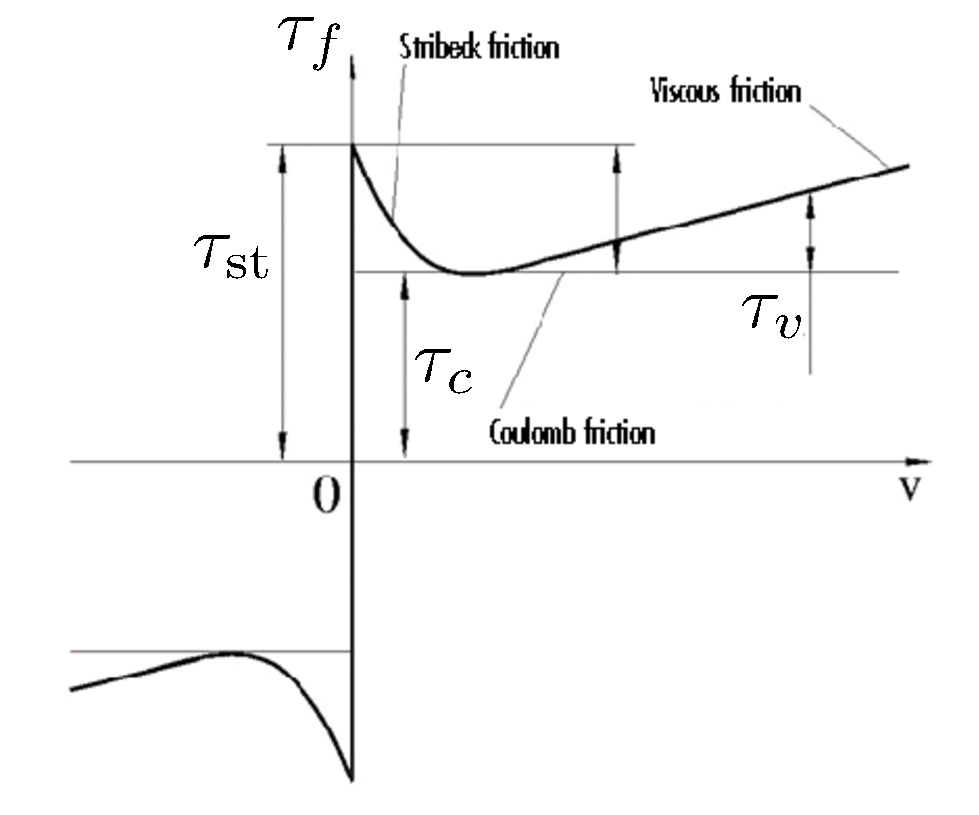
\includegraphics[width=0.5\textwidth]{Figures/Stribeck}}
	\caption{Friction Torque Model - Reference~\cite{OLSSON1998176}}
	\label{fig:Stribeck}
\end{figure}

The friction model used for reaction wheels uses a combination of static, Coulomb, and viscous friction and can be seen in Fig.~\ref{fig:Stribeck}. To incorporate all of these effects, the friction was adopted using the Stribeck friction model seen in Reference~\cite{OLSSON1998176}. The following equation describes the calculation of the friction torque on the reaction wheels.

\begin{equation}
\tau_{f} = - \sqrt{2 e} (\tau_{\text{st}}-\tau_c) e^{\Big[-\big(\frac{\Omega}{\beta_{\text{st}}}\big)^2\Big]} - \tau_c \tanh \Big[\frac{10 \Omega}{\beta_{\text{st}}}\Big] - c_v \Omega
\label{eq:friction}
\end{equation}

In Eq.~\eqref{eq:friction}, $\tau_{f}$ is the friction torque, $\tau_{\text{st}}$ is the static friction magnitude, $\tau_c$ is the coulomb friction magnitude, $\beta_{\text{st}}$ is the Stribeck coefficient which modifies the peakedness of the Stribeck curve, and $c_v$ is the viscous damping coefficient. These variables can also be seen in the variable descriptions in Fig.~\ref{fig:Stribeck}. 

The Stribeck function is only applicable when the reaction wheel is starting from rest. In contrast, when the reaction wheel starts from a non-zero speed, or has already broken free of static friction term, then the following equation is implemented:

\begin{equation}
\tau_{f} = - \tau_c \text{sgn} (\Omega) - c_v \Omega
\label{eq:friction2}
\end{equation}
This logic and math is implemented in the reaction wheel dynamics module. 
